\documentclass[10pt,conference,compsocconf]{IEEEtran}

%\usepackage{times}
%\usepackage{balance}
\usepackage{url}
\usepackage{graphicx}	% For figure environment
\usepackage{listings} 

\usepackage{amsmath}
\usepackage[utf8]{inputenc}
\usepackage[T1]{fontenc}
\usepackage{textcomp}
\usepackage{gensymb}

\lstset{language=Python} 


\begin{document}
\title{Preprocessing of High-Resolution Satellite Imagery for subsequent \\Segmentation using Convolutional Neural Networks}

\author{
 Balz Guenat \& Lukas Bischofberger\\
  Department of Computer Science, ETH Zurich, Switzerland
}

\maketitle

\begin{abstract}
  
\end{abstract}

\section{Introduction}
Image segmentation is a classic computer vision problem. But the reappearance of neural networks also made this problem interesting in new dicipline, the convolutional neural network (CNN). We tackle the problem of road segmentation in images taken from Google Maps with a CNN. Therefore we developed a new pipeline based on CNN, coupled with pre- and postprocessing to solve the challenging task. Our approach makes it's main contribution with a preprocessing and sample generation method.

\section{Models and Methods}
First we preprocess the images to obtain more additional information which is not captured in RGB image data. Section .. explains the different methods we tried.
Then we divided the image in patches of different sizes. We tried different parameters (2,4,8,16,32) for the patch size resulting in different coarseness levels. Section .. will explain how specifically an individual patch has been generated. Those patches are packed into batches and fed into the CNN whose configuration is further detailed in section ... Finally we have developed a postprocessing method to combine predictions from different coarseness levels and remove false positives from the final prediction.

\subsection{Preprocessing}

We use different preprocessing methods to extend the input data with additional channels.
In a first step we compute the saturation $S$ and lightness $L$ for each pixel $(R,G,B) \in [0,1]^3$ according to the HSL\footnote{Hue, Saturation, Lightness coordinate representation} system as follows.
$$ Cmax := max(R,G,B) $$
$$ Cmin := min(R,G,B) $$
$$d := Cmax - Cmin$$
$$ L := \frac{Cmax + Cmin}{2} $$
\[
S :=
\begin{cases}
	0, & \text{if } d = 0\\
	\frac{d}{1-|2L-1|}, & \text{otherwise}
\end{cases}
\]
We then extend the images by these newly computed channels, such that every pixel is now comprised of 5 values $(R,G,B,S,L) \in [0,1]^5$. Figure \ref{fig:satlit} shows the resulting channels for the image shown in figure \ref{fig:original_and_truth}.

In a second step we compute texture features.
We present two different methods which we shall call the \emph{GLCM method} and the \emph{MaxDiff method}, only one of which is used in each model.
The \emph{GLCM method} utilizes the Gray-Level Co-occurrence Matrix (GLCM) \cite{glcm} as computed on the lightness channel.
Kirthika et al. \cite{kirthika2011automated} achieved good results using a very similar method.
For each pixel we compute the GLCM for an offset of 1, angles of 0° and 90° and 8 levels.
We then use this GLCM to compute the contrast, correlation, energy and homogeneity features of the pixel, yielding 4 additional channels which we append to the pixel.
Using this method, the preprocessed images are comprised of 9 channels $(R,G,B,S,L,T1,T2,T3,T4)$.
Figure \ref{fig:preproc_glcm} shows the resulting channels.
The \emph{MaxDiff method} is a more lightweight alternative to the above.
It is also computed on the lightness channel.
For each pixel $p$ and its right and lower neighbors $p_r$ and $p_d$, we compute the following contrast channel and append it to the pixel.
$$ T := max(|p-p_r|,|p-p_d|) \in [0,1] $$
Using this method, the preprocessed images are comprised of 6 channels $(R,G,B,S,L,T)$.
Figure \ref{fig:preproc_simple} shows the resulting channel.

\begin{figure}
	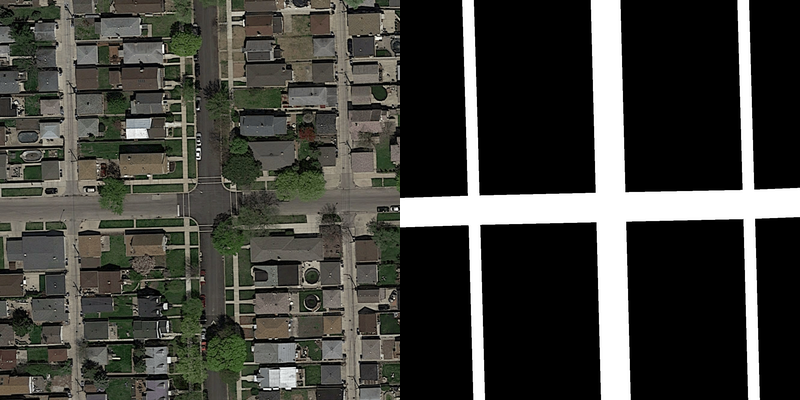
\includegraphics[width=\columnwidth]{pictures/original_and_truth}
	\caption{Original image and manually set labels}
	\label{fig:original_and_truth}
\end{figure}
\begin{figure}
	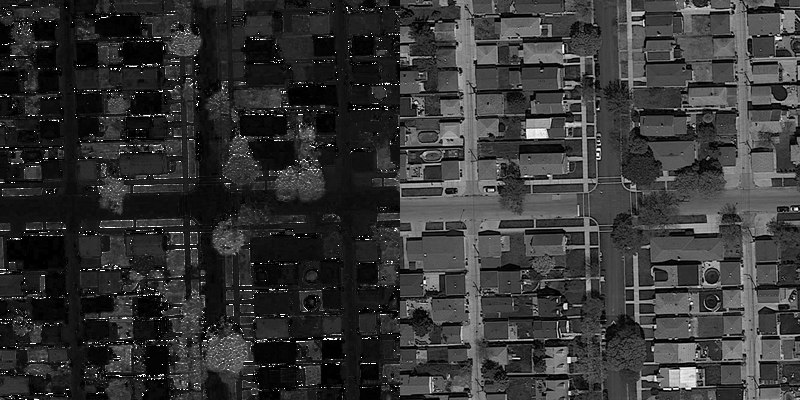
\includegraphics[width=\columnwidth]{pictures/saturation_and_lightness}
	\caption{Saturation and lightness channels, computed in preprocessing step 1.}
	\label{fig:satlit}
\end{figure}
\begin{figure}
	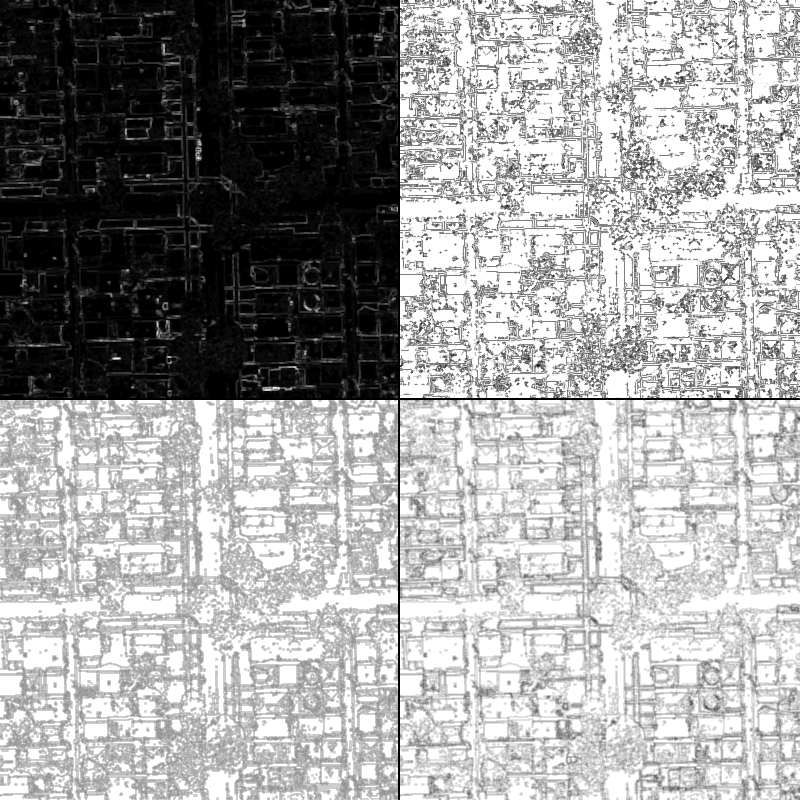
\includegraphics[width=\columnwidth]{pictures/preproc1_all}
	\caption{Contrast, correlation, energy and homogeneity channels, computed in preprocessing step 2A.}
	\label{fig:preproc_glcm}
\end{figure}
\begin{figure}
	\centering
	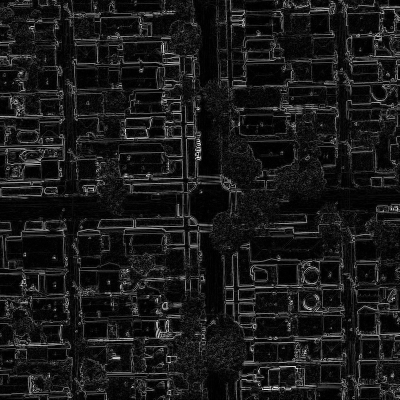
\includegraphics[width=.5\columnwidth]{pictures/preproc2}
	\caption{Contrast channel, computed in preprocessing step 2B.}
	\label{fig:preproc_simple}
\end{figure}

\subsection{CNN model}
For reasons explained below in the postprocessing sections we rely on three different CNN models each working on different patch sizes cut from the original images. They are quite similar and only differ in their number of convolutional layers and filter sizes. 
\subsubsection{Patch size 2}
	For patches with size 2 we use one convolutional layer with filter size 2x2 and 80 channels followed by a RELU and a maxpooling layer of size 2x2. 
\subsubsection{Patch size 8}
	For patches of size 8 we use two convolutional layers followed by a RELU and a maxpooling layer each. The first convolutional layer has filter size 4x4. The second filter has size 2x2, they have 200 and 400 channels respectively. 
\subsubsection{Patch size 16}
    For the largest patches we use three convolutional layers all followed by a RELU and a maxpooling layer. The first two convolutional layers have filter size 4x4. The last filter has size 2x2, they have 200, 300 and 400 channels respectively. 
    
The convolutional layers are followed by two fully connected layers with depth 1200, there we also included dropout to avoid overfitting. To train the network we used the AdamOptimizer \cite{adam} with an exponentially decaying learning rate.

    
\subsection{Postprocessing}
As stated above we developed different models with changing patch sizes. These make all predictions which have their advantages. For example a CNN with patch sizes 2 can accurately predict small areas, this is specifically useful for removing false positives as e.g. green areas of tress should not be predicted as road if they're not covering the road. On the other hand with small patch sizes our model is not able to distinguish between a rooftop and a road which are both gray. Therefore we also need the bigger context to avoid these kind of false positives. In the postprocessing we are combining the predictions of models with patch sizes of [2,8,16] pixels. A final prediction of a pixel is classified as road if the sum of the predictions over the different patch sizes is above a certain threshold. We calculate the predictions of all patches with size 16 (submission size) independently for the different predictions, then we sum them up and classify only the submission patch sizes. See the following equation where $x$ and $y$ are the pixel coordinated in an image and $i$ and $j$ are the pixel coordinates in a patch.

\[
pr(x,y) :=
\begin{cases}
	1 & \text{if} \sum_{s={2,8,16}} \mean[pr(i,j,s)] > threshold\\
	0 & \text{otherwise}
\end{cases}
\]


\section{Evaluation}
First we show how our preprocessed data performs in comparison to non augmented data and how different new features affect the prediction accuracy. Then we compare our pipeline to the baseline algorithm. Further we evaluate our postprocessing method, combining the models described above. 

\subsection{Preprocessing}

Three cases: 
1 w/o data augmentation.
2 with saturation and lumination
3 with edge detection
4 with texture from literature

\subsection{Baseline comparison}
The baseline algorithm based on CNN was trained on 60 image and evaluated on a validation set of 10 images. We trained our pipeline on the same data and show the resulting errors in \ref{fig:baseline}. 

\begin{figure}
	\centering
	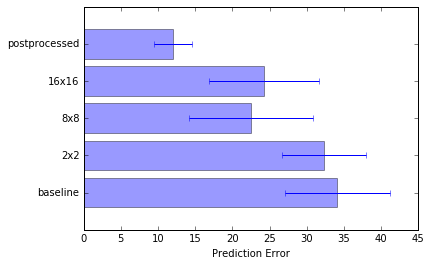
\includegraphics[width=.8\columnwidth]{pictures/baseline}
	\caption{Mean errors of different patch sizes, postprocessed and baseline}
	\label{fig:baseline}
\end{figure}

For the second baseline algorithm we trained it on 60 images again and predicted the one in figure \ref{fig:scikit} for comparison to our pipeline.

\begin{figure}
	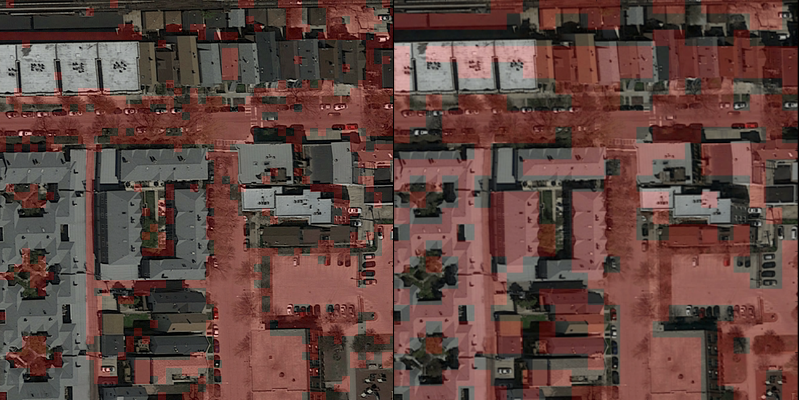
\includegraphics[width=\columnwidth]{pictures/baseline1-comp}
	\caption{Our model (left) and prediction of baseline algorithm using logistic regression (right)}
	\label{fig:scikit}
\end{figure}

\subsection{Postprocessing}
We ran the model described above with the following configuration for the three patch sizes. 
\begin{lstlisting}
EPOCHS = 10
TRAINING_SIZE = 60
VALIDATION_SIZE = 10
BATCH_SIZE = 63
NUM_CHANNELS = 3
\end{lstlisting}
For all the models we calculated the error on the validation set. Then we ran the postprocessing on the validation predictions with varying thresholds and calculated the error on the new predictions. See the results in figure \ref{fig:postprocessing} where we used thresholds between 2 and 3.2. Unfortunately the error doesn't decrease anymore while increasing the threshold. Also the optimal threshold for test data does not equal the one for validation data.

\begin{figure}
	\centering
	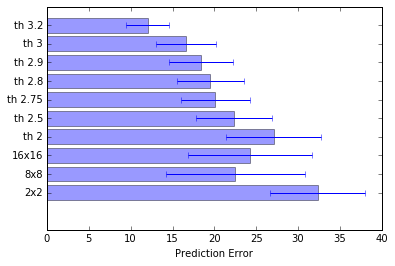
\includegraphics[width=.8\columnwidth]{pictures/postprocessing}
	\caption{Mean errors of different patch sizes and postprocessed predictions with variying threshold}
	\label{fig:postprocessing}
\end{figure}


\section{Discussion}

Our evaluation of the postprocessing shows that we can reliably combine different models which are run independently to gain better predictions. Unfortunately this approach relies on the theory that the different models have different strengths. If in any case no model is able to detect a certain structure the postprocessing won't help either. So in future research we would investigate in how to train model with certain strengths.


\section{Summary}
Our paper makes two main contributions, we show different data augmentation schemes in the preprocessing section which allows us to recognize more information from the data than given initially. Because our focus was not specifically set on the convolutional neural network its architechture is fairly common and wasn't enhanced much. The greater focus was set on the postprocessing to combine different non-perfect results to gain better predictions. We think that we could show, that using several simple and thus quite fast and parallelizable models, we could get better performance that we got using one more complex model.

\bibliographystyle{IEEEtran}
\bibliography{balu}
\end{document}
